\chapter{Supplementary Results} % Main appendix title
\label{app:suppresults}
\section{Semantic Embeddings}
\subsection{Principle Component Analysis of Embeddings}

To examine the internal structure of different embeddings, we performed PCA and plot the eigenvalues of each PC. Refer to Figure \ref{fig:EngDecorVarRatio} for English spaces, Figure \ref{fig:FreDecorVarRatio} for French ones. 

\begin{figure}
    \centering
    \makebox[\linewidth]{
    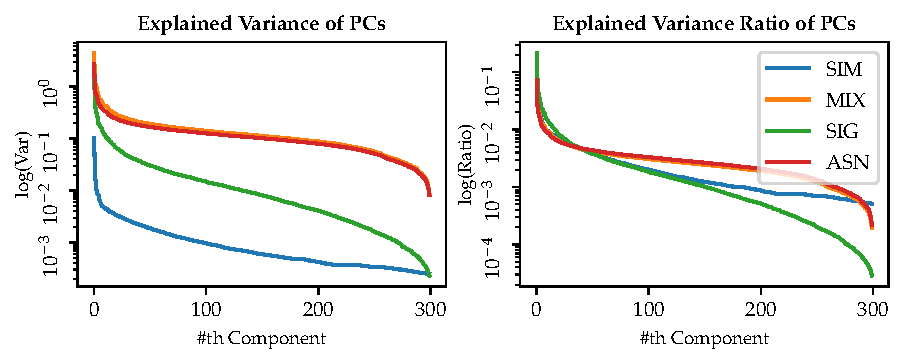
\includegraphics[scale=.8]{Figures/EngDecorVarRatio.pdf}
    }
    \caption[EVR of 4 Semantic Spaces, English]{PCA of 4 English semantic spaces of lexicon size 8157. \textbf{Left panel}: The projected \code{SIM} onto \code{MIX} (\code{SIG}) has larger variance than \code{SIM}. The suppression of \code{SIG} from \code{MIX} has little impact on \code{MIX}'s variance. \textbf{Right panel}: \code{SIG} and \code{SIM} have a denser variance concentrated on first PCs, while \code{ASN} and \code{MIX} have more homogeneous variance distributions. These are indications that \code{ASN} and \code{MIX} possess rich semantic information compared to \similarity spaces.} 
    \label{fig:EngDecorVarRatio}
\end{figure}
\begin{figure}
    \centering
    \makebox[\linewidth]{
    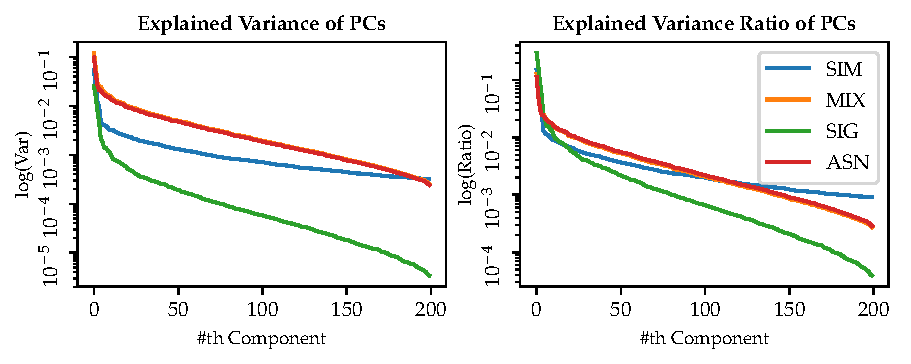
\includegraphics[scale=0.8]{Figures/FreDecorVarRatio.pdf}
    }
    \caption[EVR of 4 Semantic Spaces, French]{PCA of 4 French semantic spaces of lexicon size 24519. \textbf{Left panel}: Due to the poor linear correlation found between \code{SIM} and \code{MIX}, the variance of \code{SIG} is systematically smaller than the other three spaces, the original space \code{SIM} has larger variances. The suppression of \code{SIG} from \code{MIX} has little impact on the model's variance. \textbf{Right panel}: \code{SIG} has a denser variance concentrated on first PCs, while the other three spaces have more homogeneous variance distributions.\label{fig:FreDecorVarRatio}} 

\end{figure}


\subsection{Visualization of Semantic Spaces}
\label{appsubsec:projectorvisu}

The English \code{SIM}, French \code{SIM} and \code{ASN} spaces are visualized with Tensorflow Embedding Projector. While the English \code{SIM} (Figure \ref{fig:engSIMwalk}), built with \code{WordNet}, is still homogeneously distributed in the span of the first 3 principle vectors, the French \code{SIM} (Figure \ref{fig:freSIMmarcher}) is dominated by POS information. The four first PCs each denotes the dimension of nouns, verbs, adjectives and adverbs. Despite the data source of French \code{WOLF} being \code{WordNet}s of other languages, many of the semantic links are lost.

French \code{ASN} (Figure \ref{fig:freASNmarcher}) on the contrary, has no substantial influence by POS. 

\begin{figure}
    \centering
    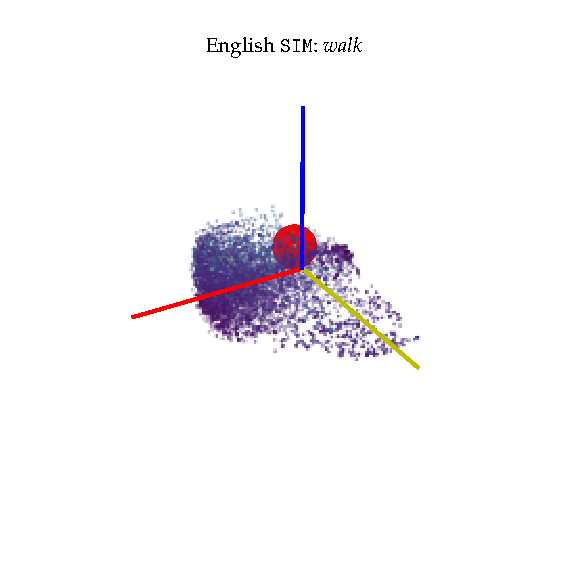
\includegraphics[clip, trim=1cm 1.5cm 2cm 0.2cm, scale=1]{Figures/EngSIMPCAforwalk.pdf}
    \caption[English \code{SIM} Space Visualization]{Each point represent a word, coordinated in the first 3 PC of the English \code{SIM} space. The points are regularly distributed in a sphere, with several local clusters centered by POS tags. The red sphere is the location of \emph{walk}. The color gradient denotes the vectorial proximity of the words with \emph{walk}. Lighter colors denotes a larger similarity.}
    \label{fig:engSIMwalk}
\end{figure}

\begin{figure}
    \centering
    \begin{minipage}[t]{.5\textwidth}
        \centering
        \makebox[.5\linewidth]{
        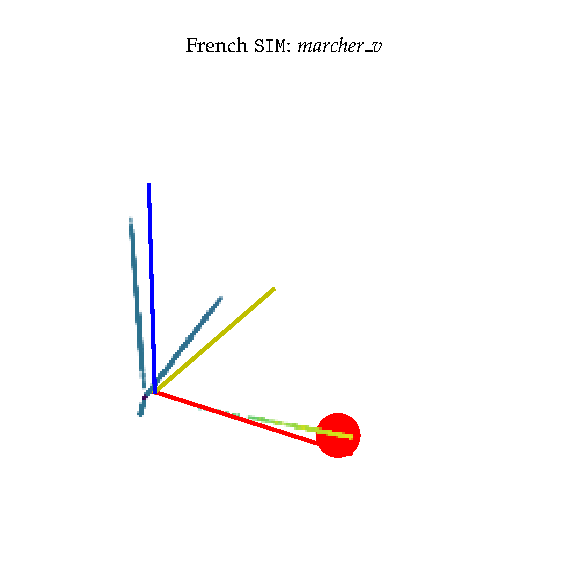
\includegraphics[clip, trim=1cm 1.5cm 2cm 0.2cm, scale=1]{Figures/FreSIMPCAformarcher_v.pdf}
        }
        \caption[French \code{SIM} Space Visualization]{Due to the nature of \code{WOLF}, 
        \code{SIM}'s first PCs denotes POS category. Light colors indicate the proximity of the represented words with \emph{marcher\_v}. All of the semantic neighbours of \emph{marcher} are verbs.}
        \label{fig:freSIMmarcher}
    \end{minipage}%
    \begin{minipage}[t]{.5\textwidth}
        \centering
        \makebox[.5\linewidth]{
        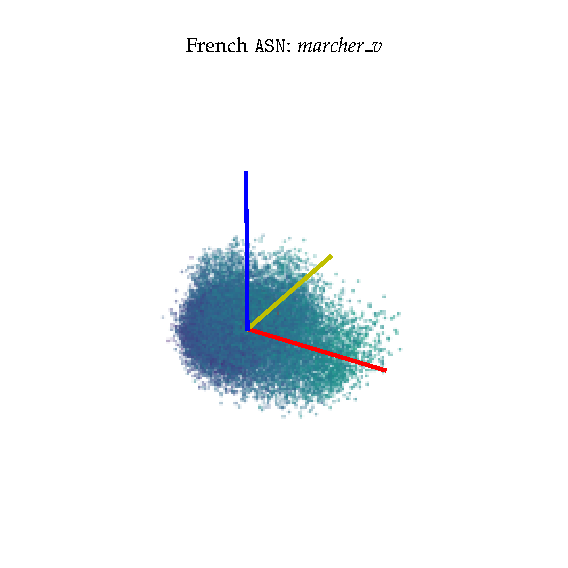
\includegraphics[clip, trim=1cm 1.5cm 2cm 0.2cm, scale=1]{Figures/FreASNPCAformarcher_v.pdf}
        }
        \caption[French \code{ASN} Space Visualization]{\code{ASN}'s variance are more homogeneously distributed over PCs.}
        \label{fig:freASNmarcher}
    \end{minipage}
\end{figure}

\subsection{Semantic Ranking Task Results}
\label{appsubsec:wnembeddingtests}

In the first stage of the project, we tested different combinations of semantic relations to maximize \similarity scores while minimize \association. The different iteration scores are reported in Table \ref{apptab:engWordNetIteration}. 

Along the trials with \code{WordNet}, another synonym database created based on thesauri is also tested with the same algorithm. The word-pair proximity ranking task indicates that associational relations can still be deducted from the synonyms. However, the \textbf{SIMLEX-999} score reported by this data source approaches the state-of-the-art of single-source language models\footnote{Task dashboard: \url{https://fh295.github.io/simlex.html}.}. 

\begin{table}
 \centering
 \begin{ThreePartTable} 
\begin{tabularx}{\textwidth}{p{3cm} *{2}{p{.5cm}} *{2}{p{1.7cm}} *{4}{L}} 
\multicolumn{8}{l}{\tabhead{English \code{WordNetEmbedding} Iterations}} \\
 \toprule
 \mr{2}{=}{\tabhead{Relations}} & \mr{2}{=}{\rotatebox[origin=c]{90}{\tabhead{Lexicon}}} & \mr{2}{=}{\rotatebox[origin=c]{90}{\tabhead{Dim.}}} & \mr{2}{=}{\tabhead{Metric}}  & \mc{3}{l}{\tabhead{\emph{Similarity}}} & \tabhead{\emph{Association}} \\
 \cmidrule{5-7}
 & & & & \small{\textbf{SIMLEX-999}} & \small{\textbf{WS353-SIM}} & \small{\textbf{RG1965}} & \small{\textbf{WS353-ASN}} \\
 \toprule
 \mr{4}{=}{\textbf{S}ynonymy} &\mr{2}{=}{15k}  & \mr{12}{=}{850} & Pearson & .2256 & .2679 & .3627 & .123 \\
 & & & Spearman & .2001 & .2003 & .3403 & .0971 \\
\cmidrule{2-2} \cmidrule{4-8}
  & \mr{2}{=}{60k} &  & Pearson & .234 & .2112 & .3394 & .1449 \\
 & & & Spearman & .1747 & .1895 & .2629 & .1129 \\
 \cmidrule{1-2} \cmidrule{4-8}
 \mr{2}{=}{S+Antonymy} & \mr{6}{=}{15k} &  & Pearson & .1534 & .2743 & .373 & .0969 \\
 & & & Spearman & .1255 & .1922 & .3302 & .0817 \\
 \cmidrule{1-1} \cmidrule{4-8}
 \mr{2}{=}{S+\textbf{H}yp\textbf{e}r/\textbf{H}yp\textbf{o}nymy} &  &  & Pearson & .3904 & .4825 & .6187 & .0373 \\
 & & & Spearman & .4018 & .3856 & .5145 & .0259 \\
 \cmidrule{1-1} \cmidrule{4-8}
 \mr{6}{=}{SHeHo+ adj.participle\_of\_verb+ adj.similar+ adv.derive\_from\_adj} &  &  & Pearson & .5079 & .5333 & .6784 & .0525 \\
 & & & Spearman & .4986 & .4214 & .576 & .0272 \\
 \cmidrule{2-2} \cmidrule{4-8}
  & \mr{2}{=}{60k} &  & Pearson & .5268 & .5483 & .6991 & .1092 \\
 & & & Spearman & .5152 & .4757 & .5501 & .0515 \\
 \cmidrule{2-8}
  & \mr{2}{=}{15k\tnote{0}}  & \mr{2}{=}{511} & Pearson & .506 & & & .0279 \\
 & & & Spearman & .4989 & & & .0193 \\
 \cmidrule{2-8} 

&  & \mc{2}{r}{Out Of Vocabulary} & .002 & .02 & 0 & .012 \\
\midrule
\mr{4}{=}{All\tnote{1}} & \mr{2}{=}{13k\tnote{2}} & \mr{8}{=}{850} & Pearson & .5 & .65 & .65 & .32 \\
 & & & Spearman & .52 & .67 & .75 & .33 \\
\cmidrule{2-2} \cmidrule{4-8}
 & \mr{2}{=}{60k\tnote{3}} & & Pearson & .5 & .51 & .56 & .31 \\
 & & & Spearman & .51 & .58 & .72 & .3 \\
\cmidrule{1-2} \cmidrule{4-8}
 \mr{3}{=}{Synonym Database\tnote{4}} & \mr{2}{=}{60k\tnote{5}} &  & Pearson & .6814 & .5819 & .8155 & .317 \\
 & & & Spearman & .6566 & .4677 & .7032 & .3153 \\
 \cmidrule{2-8}
 & & \mc{2}{r}{Out Of Vocabulary} & .066 & .227 & .077 & .19 \\
\bottomrule
\end{tabularx}
\begin{tablenotes}
    \footnotesize
    \item[0] Version reported in Table \ref{tab:engdecorrelationscores}.
    \item[1] Data reported by \textcite{saediWordNetEmbeddings2018}.
    \item[2] Cue words selected from psycholinguistic experiment datasets.
    \item[3] Words selected randomly. On the contrary, our implementation selects the top 60k most frequent words in \code{WordNet}. 
    \item[4] Synonym database is created by thesauri fusion and symmetrization. Data provided by \textcite{plouxModelMatchingSemantic2003}.
    \item[5] The synonym database contains multi-word phrases, whereas task benchmarks only test for single-word pairs. The actual lexicon size of the database is 36718.
\end{tablenotes}
\end{ThreePartTable}
\caption[English \code{WordNetEmbedding} Iterations]{Placeholder \label{apptab:engWordNetIteration}}
\end{table}

% \begin{table}
%     \centering
%     \begin{ThreePartTable} 
%    \begin{tabularx}{\textwidth}{p{3cm} *{3}{R} *{4}{L}} 
% \multicolumn{8}{l}{\tabhead{English Dissociation}} \\
%  \toprule
%  \mr{2}{=}{Common Crawl} & 2.2M, cased & 300 & Pearson & .3946 & .6573 & .6812 & .6091 \\
%  & & & Spearman & .3752 & .6298 & .6577 & .5709 \\
%  & & & OOV & .1 & 0 & 0 & 0 \\
%  \mr{2}{=}{CommonCraw - 01-23 Sim} & 8157 & 300 & Pearson & .1953 & .5854 & .5547 & .5633 \\
%  & & & Spearman & .2133 & .5719 & .5641 & .5918 \\
%  & & & OOV & & & & \\
%  \bottomrule
% \end{tabularx}
% \end{ThreePartTable}
% \caption[English Semantic Space Dissociation]{Placeholder \label{apptab:engDissociation}}
% \end{table}

\subsection{Example of Semantic Neighbours in French Embeddings} 

No systematic control for \code{ASN} is performed for the \citetitle{desaint-exuperyPetitPrince1943} story. We taken several examples and examined the semantic neighbours with Tensorflow Projector. Table \ref{tab:freNeighbour} gives an example and nature of the semantic neighbours in four embedding spaces conforms with the hypothesized properties of the semantic principles (syntagmatic and paradigmatic).

\begin{table}
    \centering
    \begin{tabularx}{\textwidth}{*{4}{P{.23\textwidth}}}
    \mc{4}{l}{\tabhead{French Semantic Embeddings}} \\
    \mc{4}{l}{\tabhead{Target word:} professeur\_n} \\
    \toprule
    \code{SIM} & \code{SIG}& \code{ASN} & \code{MIX} \\
    \toprule
    pédagogue\_n & pédagogue\_n & fondateur\_n & naissance\_n\\
éducateur\_n & éducateur\_n & psychose\_n & psychose\_n\\
instituteur\_n & instructeur\_n & éducation\_n & éducation\_n\\
instructeur\_n & instituteur\_n & serveur\_n & secrétaire\_n\\
\cmidrule{2-2}

arbitre\_n & arbitre\_n & secrétaire\_n & logique\_a\\
lecteur\_n & adjudant\_n & défenseur\_n & fondateur\_n\\
enseignant\_n & passe\_n & imitation\_n & chronique\_a\\
\cmidrule{1-1}

passe-partout\_n & passe-partout\_n & vicaire\_n & imitation\_n\\
passepartout\_n & lecteur\_n & sensation\_n & sensation\_n\\
passe\_n & enseignant\_n & protecteur\_n & honneur\_n\\
adjudant\_n & abonné\_n & protectionnisme\_n & traumatisme\_n\\
aide\_de\_camp\_n & maestro\_n & volontaire\_n & vicaire\_n\\
maître\_n & spécialiste\_n & fonctionnaire\_n & facilité\_n\\
maestro\_n & châtelain\_n & naissance\_n & serveur\_n\\
capitaine\_de\\ \_vaisseau\_n & capitaine\_n & photographie\_n & proposition\_n\\
maître\_d'hôtel\_n & commandant\_n & producteur\_n & disparition\_n\\
commandant\_n & propriétaire\_n & évidence\_n & moteur\_n\\
capitaine\_n & professionnel\_n & honneur\_n & sagesse\_n\\
spécialiste\_n & leader\_n & croisade\_n & croisade\_n\\
commandement\_n & contributeur\_n & missionnaire\_n & évidence\_n\\
abonné\_n & possesseur\_n & moteur\_n & quantité\_n\\
overlord\_n & savant\_n & pluralisme\_n & défaillance\_n\\
châtelain\_n & commandement\_n & sagesse\_n & édition\_n\\
précepte\_n & acquéreur\_n & coexistence\_n & défenseur\_n\\
fondateur\_n & acheteur\_n & objectif\_a & volontaire\_n\\
débutant\_n & participant\_n & facilité\_n & protecteur\_n\\
tyro\_n & officiel\_n & disparition\_n & pluralisme\_n\\
\bottomrule
    \end{tabularx}
    \caption[Exemplar Neighborhoods in French Semantic Embeddings]{The vectorial distances are computed on the whole original vector space. Words are sorted on the ascending vectorial distance. Lines are drawn at the limit of synonyms. \label{tab:freNeighbour}}
    
    \end{table}


\subsection{Vocabulary Coverage by POS}

Additional fMRI encoding regressions have been trained with POS-specific design matrices to reveal potential differences of semantic processing. The statistics for the POS-specific corpus is reported in Table \ref{apptab:lppcoverage}.
\begin{table}
    \centering
    \begin{ThreePartTable}  
    \begin{tabularx}{\textwidth}{L *{10}{R}}
    \multicolumn{11}{l}{\tabhead{The Little Prince Vocabulary Coverage}} \\
    \toprule
    &  & \multicolumn{9}{l}{\tabhead{\# Instances in fMRI Recording Session}} \\
    \toprule
    &  & \tabhead{R1} & \tabhead{R2} & \tabhead{R3}& \tabhead{R4}& \tabhead{R5}& \tabhead{R6}& \tabhead{R7}& \tabhead{R8}& \tabhead{R9}\\
    \toprule
    \multicolumn{11}{l}{\tabhead{Nouns}} \\
    \toprule
    \mr{2}{*}{Story} & \textbf{T} &  269 & 286 & 306 & 242 & 284 & 355 & 281 & 265 & 246 \\
     & \textbf{V} & 142 & 140 & 152 & 107 & 108 & 147 & 109 & 135 & 121 \\
    \midrule
    \mr{4}{*}{\parbox{0.8cm}{\code{SIM} 56665}} & TM & 17 & 3 & 7 & 5 & 14 & 14 & 11 & 11 & 16 \\
     & \% & 6.32 & 1.05 & 2.29 & 2.07 & 4.93 & 3.94 & 3.91 & 4.15 & 6.50 \\
     & VM & 10 & 3 & 6 & 3 & 3 & 8 & 6 & 7 & 7 \\
     & \% & 7.04 & 2.14 & 3.95 & 2.80 & 2.78 & 5.44 & 5.50 & 5.19 & 5.79 \\
    \midrule
    \mr{4}{*}{\parbox{0.8cm}{\code{ASN} /\code{MIX} /\code{SIG} 24519}} & TM & 20 & 9 & 8 & 10 & 22 & 16 & 11 & 13 & 17 \\
     & \% & 7.43 & 3.15 & 2.61 & 4.13 & 7.75 & 4.51 & 3.91 & 4.91 & 6.91 \\
     & VM & 12 & 5 & 7 & 4 & 7 & 10 & 6 & 8 & 8 \\
     & \% & 8.45 & 3.57 & 4.61 & 3.74 & 6.48 & 6.80 & 5.50 & 5.93 & 6.61 \\
     \toprule
    \multicolumn{11}{l}{\tabhead{Verbs}} \\
    \toprule
    \mr{2}{*}{Story} & \textbf{T} & 227 & 274 & 313 & 306 & 258 & 296 & 331 & 278 & 335 \\
     & \textbf{V} & 104 & 109 & 142 & 119 & 84 & 113 & 99 & 110 & 118 \\
    \midrule
    \mr{4}{*}{\parbox{0.8cm}{\code{SIM} 56665}} & TM & 9 & 15 & 14 & 15 & 10 & 4 & 7 & 12 & 7 \\
     & \% & 3.96 & 5.47 & 4.47 & 4.90 & 3.88 & 1.35 & 2.11 & 4.32 & 2.09 \\
     & VM & 7 & 7 & 9 & 11 & 9 & 4 & 5 & 8 & 6 \\
     & \% & 6.73 & 6.42 & 6.34 & 9.24 & 10.71 & 3.54 & 5.05 & 7.27 & 5.08 \\
    \midrule
    \mr{4}{*}{\parbox{0.8cm}{\code{ASN} /\code{MIX} /\code{SIG} 24519}} & TM & 9 & 19 & 15 & 17 & 10 & 8 & 9 & 12 & 14 \\
     & \% & 3.96 & 6.93 & 4.79 & 5.56 & 3.88 & 2.70 & 2.72 & 4.32 & 4.18 \\
     & VM & 7 & 10 & 10 & 13 & 9 & 7 & 6 & 8 & 10 \\
     & \% & 6.73 & 9.17 & 7.04 & 10.92 & 10.71 & 6.19 & 6.06 & 7.27 & 8.47 \\
     \toprule
     \multicolumn{11}{l}{\tabhead{Adjectives \& Adverbs}} \\
     \toprule
     \mr{2}{*}{Story} & \textbf{T} & 229 & 252 & 241 & 214 & 190 & 251 & 207 & 169 & 221 \\
     & \textbf{V} & 102 & 111 & 117 & 103 & 100 & 107 & 94 & 83 & 104 \\
     \midrule
     \mr{4}{*}{\parbox{0.8cm}{\code{SIM} 56665}} & TM & 10 & 12 & 11 & 7 & 6 & 15 & 6 & 7 & 4 \\
      & \% & 4.37 & 4.76 & 4.56 & 3.27 & 3.16 & 5.98 & 2.90 & 4.14 & 1.81 \\
     & VM & 9 & 6 & 7 & 6 & 4 & 7 & 5 & 4 & 3 \\
     & \% & 8.82 & 5.41 & 5.98 & 5.83 & 4.00 & 6.54 & 5.32 & 4.82 & 2.88 \\
     \midrule
     \mr{4}{*}{\parbox{0.8cm}{\code{ASN} /\code{MIX} /\code{SIG} 24519}} & TM & 19 & 19 & 15 & 10 & 16 & 36 & 15 & 12 & 10 \\
      & \% & 8.30 & 7.54 & 6.22 & 4.67 & 8.42 & 14.34 & 7.25 & 7.10 & 4.52 \\
      & VM & 11 & 11 & 9 & 8 & 10 & 15 & 8 & 6 & 7 \\
      & \% & 10.78 & 9.91 & 7.69 & 7.77 & 10.00 & 14.02 & 8.51 & 7.23 & 6.73 \\
    \bottomrule
    \end{tabularx}
    \end{ThreePartTable}
    \caption[The Little Prince Vocabulary Coverage by POS]{\textbf{T}: Token, \textbf{V}: Lexicon Unit, M: Miss\label{apptab:lppcoverage}}
    \end{table}


\section{Non-nested Model Comparison}
\label{appsubsec:nonnestedcompres}

\subsubsection{Use \code{SIM} to Predict \code{ASN}}

\begin{figure}
    \centering
        \makebox[.5\linewidth]{
            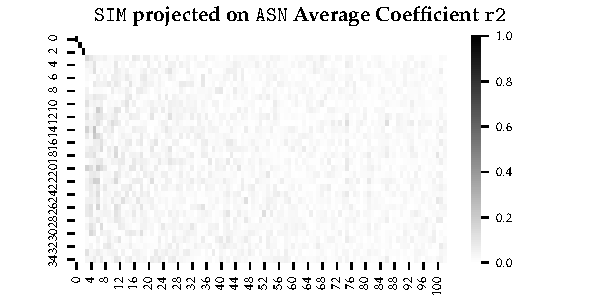
\includegraphics[scale=.8]{Figures/SIM_ASN_MODEL_COMP.pdf}
            }
            \caption[Coefficients of \texttt{SIM} Columns Predicting \texttt{ASN}]{The most effective column-models of \code{ASN} are positioned as posterior as 47, 47 then 30. Only first 35 dimensions including 3 shared non-embedding ones are visualized. No particular significant column-to-column correlation is suggested by the coefficients.} 
            \label{fig:SIMASNMODELCOMP}
\end{figure}

Each of the 203 columns in the \code{ASN} class design matrix (including non-semantic features) are predicted by 103 columns of the \code{SIM} class design matrix. The average trained coefficients are plotted in Figure \ref{fig:SIMASNMODELCOMP}. We averaged the \code{r2} score of each column model across 9 cross-validation runs. The histogram of the scores are plotted in Figure \ref{fig:SIMASNDist}, informative model scores are presented in Table \ref{tab:SIMASNScores}. As our design-matrices are orthonormalized, columns sitting at larger indexes have a dependency on smaller-indexed columns. The first columns being bell predicted start at index 12 (to 14). Other columns are scattered up to index 47. We can therefore conclude that the predictability found are purely due to numerical coincidences.

\begin{figure}
    \centering
    \begin{minipage}[t]{.5\textwidth}
        \centering
        \makebox[.5\linewidth]{
            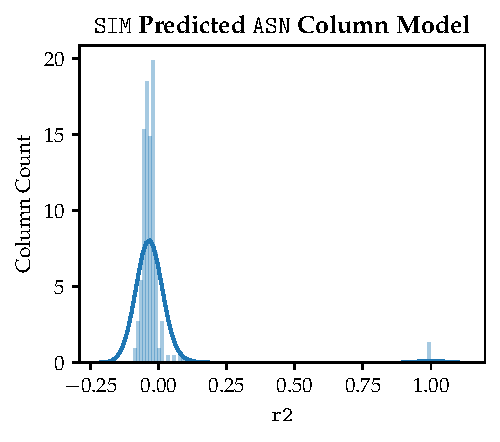
\includegraphics[scale=.8]{Figures/SIMASNDist.pdf}
            }
            \caption[\texttt{SIM} Predicted \texttt{ASN} Column Model]{3 columns are perfectly predicted as they are non-semantic features that are shared by the design matrices. For the rest most of the column-models are worse than arbitrary models.} 
            \label{fig:SIMASNDist}
    \end{minipage}%
    \begin{minipage}[t]{.5\textwidth}
        \centering
        \makebox[.5\linewidth]{
            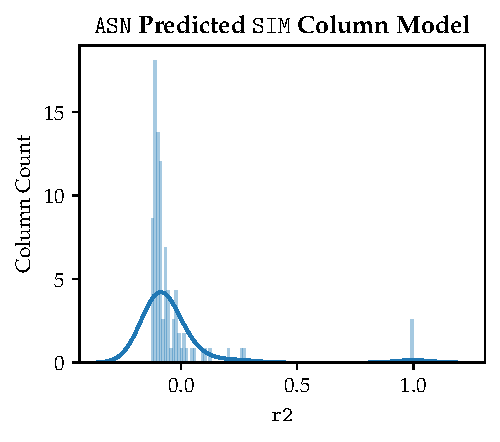
\includegraphics[scale=.8]{Figures/ASNSIMDist.pdf}
            }
            \caption[\texttt{ASN} Predicted \texttt{SIM} Column Model]{Most of the column-models are worse than arbitrary models. More columns in \code{SIM} are better predicted with \code{ASN} design matrices.} 
            \label{fig:ASNSIMDist}
    \end{minipage}
\end{figure}


\begin{table}
    \centering
    \begin{ThreePartTable}
    \begin{tabularx}{\textwidth}{p{1.7cm} *{11}{L}}
    \mc{12}{l}{\tabhead{\texttt{SIM} Predicted \texttt{ASN} Column Model Performances}} \\
    \toprule
    \tabhead{Col Index} & 22 & 20 & 14 & 37 & 47 & 18 & 27 & 26 & 13 & 12 & 30 \\ 
    \midrule 
    \tabhead{\code{r2}} & .0891 & .0834 & .0548 & .0346 & .0164 & .0152 & .0122 & .0113 & .0112 & .0075 & .0004 \\  
    \tabhead{\code{r}} & .2984 & .2887 & .2340 & .1861 & .1279 & .1233 & .1104 & .1064 & .1058 & .0867 & .0203 \\
    \bottomrule
    \end{tabularx}
    \end{ThreePartTable}
    \caption[\texttt{SIM} Predicted \texttt{ASN} Column Model Performances]{Index starts at 0, \code{ASN} group features starts from 3.  Among the 14 informative models (\code{r2} > 0), 3 are non-semantic features (not listed above). Pearson's \code{r} are converted from \code{r2}. \label{tab:SIMASNScores}}
\end{table}


\subsubsection{Use \code{ASN} to Predict \code{SIM}}

\begin{table}
    \centering
    \begin{ThreePartTable}
    \begin{tabularx}{\textwidth}{p{1.7cm} *{11}{L}}
    \mc{12}{l}{\tabhead{\texttt{ASN} Predicted \texttt{SIM} Column Model Performances}} \\
    \toprule
    \tabhead{Col Index} & 6 & 3 & 5 & 11 & 4 & 7 & 75 & 18 & 42 & 25 & 47 \\  
    \midrule 

    \tabhead{\code{r2}} & .2761 & .2646 & .2041 & .1256 & .1032 & .0971 & .0529 & .0485 & .0192 & .0158 & .0107 \\  
    \tabhead{\code{r}} & .5254 & .5144 & .4518 & .3544 & .3213 & .3116 & .2299 & .2202 & .1385 & .1256 & .1037 \\
    \bottomrule
    \end{tabularx}
    \end{ThreePartTable}
    \caption[\texttt{ASN} Predicted \texttt{SIM} Column Model Performances]{Index starts at 0, \code{SIM} group features starts from 3. \code{SIM} columns are much better predicted by \code{ASN}. \label{tab:ASNSIMScores}}
\end{table}

\begin{figure}
    \centering
        \makebox[.5\linewidth]{
            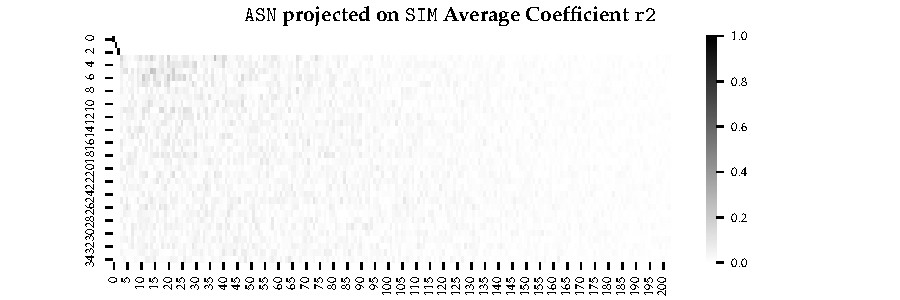
\includegraphics[scale=.8]{Figures/ASN_SIM_MODEL_COMP.pdf}
            }
            \caption[Coefficients of \texttt{ASN} Columns Predicting \texttt{SIM}]{The first 7 \code{SIM} columns are well predicted by \code{ASN} columns. The visualization suggests that the first 40 columns of \code{ASN} \emph{regressor class} correlated with the first 5 \code{SIM}-\emph{group} \emph{regressors}.} 
            \label{fig:ASNSIMMODELCOMP}

\end{figure}

The same procedure yields also 14 effective column models for \code{SIM}. The correlation coefficients are significantly higher than the models predicted with \code{SIM} matrices. Besides, the first 5 columns of \code{SIM} are all well predicted (\code{r} > 0.30) by \code{ASN}, indicating there's partial signal information overlap between the two models. Since Section \ref{appsubsec:projectorvisu} shows that the first 4 dimensions in \code{SIM} one-hot encode POS information, it is reasonable that POS information is also traceable in syntagmatic-information dominated semantic embedding.

To further investigate the column-wise correlation, we also plot the coefficients of each \code{ASN} column learned by GLM (Figure \ref{fig:SIMASNMODELCOMP}). 

\section{Regression}
\subsection{More on \(\alpha\) and Dimension Selection}
\label{appsubsec:alphadim}

\subsubsection{Completeness of Research Space}

For illustrative purpose, we selected four typical voxels in post-hoc from the regression results of \code{MIX}, run 1 subject 1 (Figure \ref{fig:TypicalVoxelDistributionS1R1})\footnote{Interactive version of the plot available online \url{https://plot.ly/~neegola/11/}.}. \code{MIX} is used since it is the default semantic space used in other works and has not been modified. Each voxel is the best modeled voxel who maximizes \code{r2} among all \(\alpha\)s using only partial feature information of a certain regressor class. For example, a \code{CWRATE} class typical voxel is a voxel of which the best \code{r2} is achieved with \emph{all} first 3 features (\code{dim=3}). 

\begin{figure}
    \centering
    \makebox[\linewidth]{
    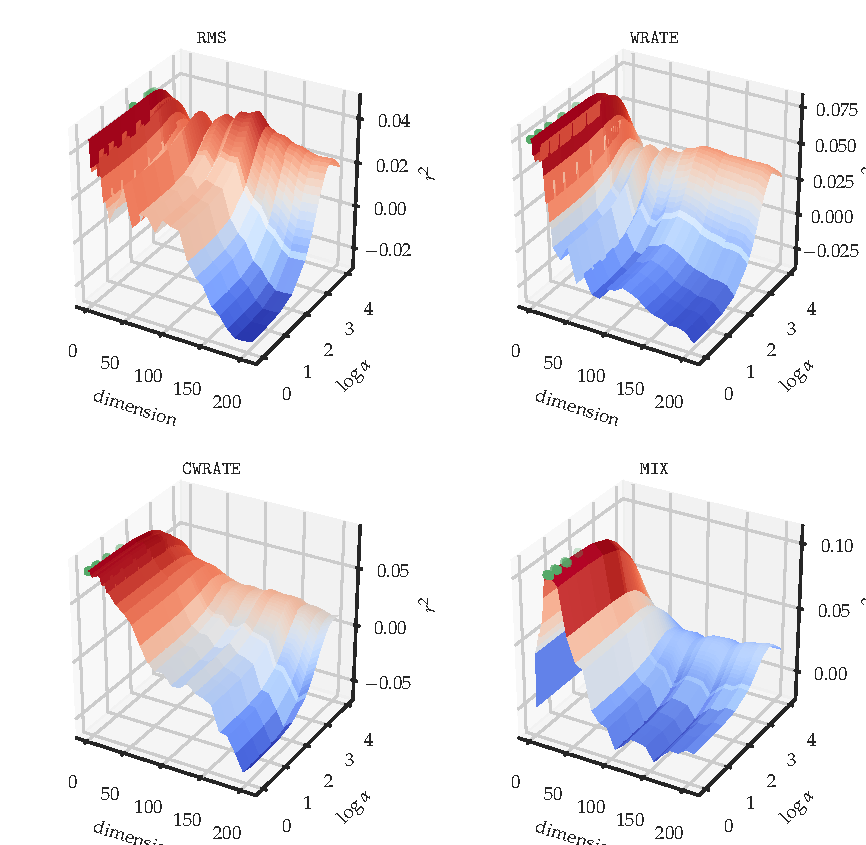
\includegraphics[scale=1]{Figures/TypicalVoxelDistributionS1R1.pdf}
    }
    \caption[Typical-Voxels' Response to \(\alpha\) and Dimension]{A selection of typical voxels found in \code{MIX} model regression results of subject 1 run 1. All trails with dimensionality and \(\alpha\) values are visualized. The title of each subplot corresponds to the voxel's best dimension profile. As shown by all four voxels, the regularization by large \(\alpha\) is beneficial only in higher feature dimensions. Our selection of \(\alpha\) contains a near-optimal value candidates for these voxels since the curve is all declining for the largest values. Green plots indicate the top 10 best configurations of the given voxel.} 
    \label{fig:TypicalVoxelDistributionS1R1}
\end{figure}

The optimal \code{r2}s of typical voxels are never attained at the upper bound of \(\alpha\) and dimension space. We plotted the heat-map for all voxels from the same run to verify if it is also the case at the whole-brain level (e.g. Figure \ref{fig:MIX_HeatmapAlphaDimS1R1}). We averaged 9 cross-validation run results to visualize subject-level best configuration distribution (Figure \ref{fig:MIX_HeatmapAlphaDimS1R0}). Histograms of best dimension and \(\alpha\) voxel-configuration of the averaged results are also plotted in Figure \ref{fig:MIX_CountPlotAlphaDimS1R0}. Plots for all runs and all subjects are available online\footnote{\code{MIX}: \url{http://bit.ly/micipsa_mix_heatmap}. \code{SIM}: \url{http://bit.ly/micipsa_sim_heatmap}. \code{SIG}: \url{http://bit.ly/micipsa_sig_heatmap}. \code{ASN}: \url{http://bit.ly/micipsa_asn_heatmap}.}. The analysis confirms that our parameter combination test range contains the near-optimal configuration for each voxel.

\begin{figure}
    \centering
    
    \makebox[.5\linewidth]{
            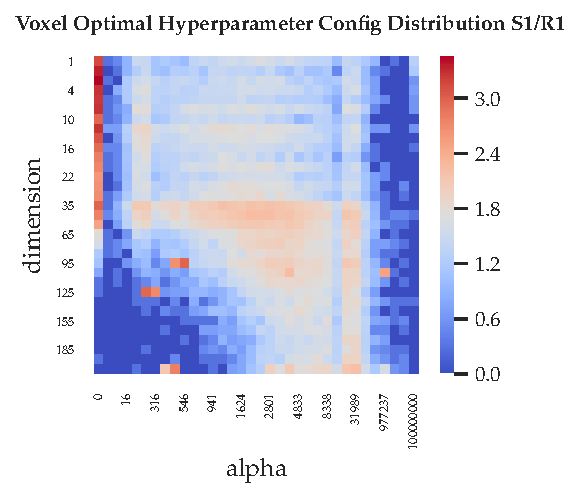
\includegraphics[scale=.8]{Figures/MIX_HeatmapAlphaDimS1R1.pdf}
            }
            \caption[Session Best Hyper-parameter Configuration Voxel-Count Heat-map]{The scores are retrieved from \code{MIX} model regression for subject 1, fMRI run 1. Each cell represents an \(\alpha\) and dimension combination. The color indicates the logarithm of number of voxels having its global optimality with a given parameter set after having filtered out non-informative voxels (\code{r2} < 0). For small dimensions (< 35), small \(\alpha\)s (including 0) achieve the best performance. Starting from dimension 35, Ridge regularization with larger \(\alpha\)s is necessary.} 
            \label{fig:MIX_HeatmapAlphaDimS1R1}
   
\end{figure}

\begin{figure}
    \centering
    \makebox[\linewidth]{
    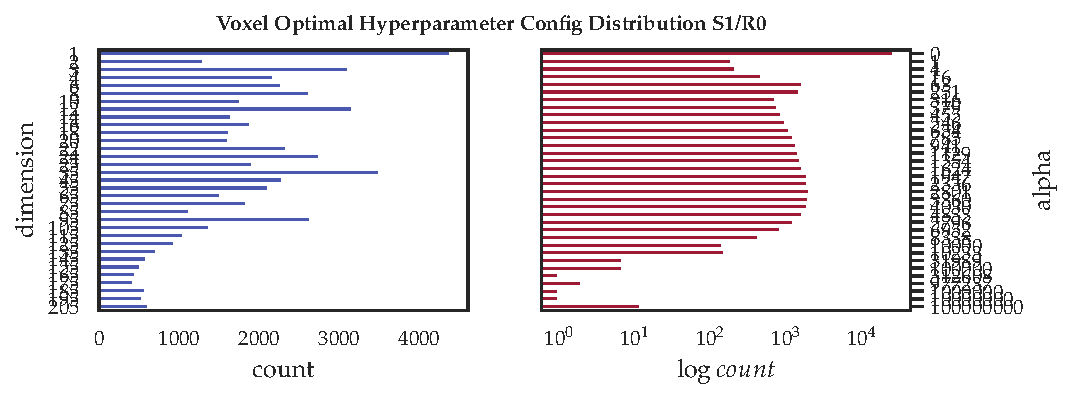
\includegraphics[scale=1]{Figures/MIX_CountPlotAlphaDimS1R0.pdf}
    }
    \caption[Best Hyper-parameter Configuration Voxel-Count Histograms]{\textbf{R0} denotes that the subject average is plotted. \textbf{Left panel}: Among informative voxels, a large portion of voxels are best modeled by \code{RMS} and \code{CWRATE} regressor classes. The addition of each semantic dimension from \code{MIX} improved a small proportion of voxel-models, marginal might be the contribution. \textbf{Right panel}: Most of the voxels are best modeled without Ridge regularization. The larger number obtained at \(\alpha=10000\) might indicate that larger alpha values might help better model a thousand voxels. A cumulation of voxel-count at the upper bound of the \(\alpha\) axis is noted: we performed post-hoc test for larger \(\alpha\) values than in the initial configuration, but the improvement of \code{r2} over the original score is marginal (\(<10^{-4}\)) for a sample of these voxels. A post-hoc analysis of larger \(\alpha\)s indicates a limited improvement of \code{r2}, thus for computational simplicity we kept the original Grid Search space of \(\alpha\).\label{fig:MIX_CountPlotAlphaDimS1R0}} 
    
\end{figure}

\subsubsection{Dimension Variability across Voxels}

At obtention of regression results, we visualized the contrast of voxel-model scores if we enforce the dimensionality of design matrix and do not perform the nested-model substitution\footnote{Histograms and scatter plots available for the first 3 runs of first 3 subjects. File name ending with \code{alpha\_best} indicates the plotted results are among the voxel-wise best alpha. \url{http://bit.ly/micipsa_dimension_variability}.}. The results indicate that fixing the semantic model dimensionality at full overfits most of the voxels.

The regularization parameter has an overall penalization effect: on increasing \(\alpha\), the overall distribution of \code{r2} is more densely centered around 0. 


\section{Embedding Model Brain Maps}
\subsection{Nested Model Cluster Tables}

For each regression model, the top 1\% and 0.1\% voxels are selected to analyze the spatial pattern of voxel-models (Table \ref{tab:rmsCluters}). 
The Wilcoxon test results for nested-model \code{r2} improvements are also clustered. The voxels are thresholded with statistical significance. Refer to Table \ref{tab:cwrateImprovementClusters} for \code{CWRATE} improvements, Table \ref{tab:simImprovementClusters} for \code{SIM}, Table \ref{tab:sigImprovementClusters} for \code{SIG} and Table \ref{tab:asnImprovementClusters} for \code{ASN}. Corresponding F-test visualization data for all nested contrasts are reported in Table \ref{tab:Ftest}.

\begin{table}
    \small
    \centering
    \begin{ThreePartTable}
    \begin{tabularx}{\textwidth}{p{1.8cm}p{.5cm}p{1.4cm}p{1cm} *{6}{r}}
    \mc{6}{l}{\tabhead{\code{RMS/CWRATE/SIM/ASN} Best Modeled Voxel Clusters}} \\
    \toprule
    \tabhead{Position} & \tabhead{BA} & \tabhead{Functional Label} & \tabhead{Feature Class} & \tabhead{x} & \tabhead{y} & \tabhead{z} & \tabhead{\#Voxel} & \code{r2} \tabhead{Peak} & \code{r2} \tabhead{Min} \\
    \toprule
    \mc{3}{l}{\tabhead{Top .1\%}} \\
    \midrule
    \mr[t]{3}{=}{Temporal Sup L} & \mr[t]{3}{=}{41} & \mr[t]{3}{=}{Prim Auditory} &  \code{RMS} &  -59 & -13 & 6 &  56 & .0362 &  .0240 \\ 
    & & & \code{CWRATE} & -61 & -12 & 4 & 61 &.0387 &  .0259\\
    & & & \code{SIM} & -60 & -13 & 6 & 53 & .0412 &  .0291 \\
    & & & \code{SIG} & -61 & -11 & 4 & 87 & .0430 & .0301\\
    & & & \code{ASN} & -60 & -13 & 6 & 53 & .0388 &  .0293 \\
    \midrule
    \midrule
    \mc{7}{l}{\tabhead{Top 1\%}}   \\
    \midrule
    \mr[t]{3}{=}{Temporal Sup L} & \mr[t]{3}{=}{41} & \mr[t]{3}{=}{Prim Auditory} & \code{RMS} & -60 & -12 & 4 & 410 & .0362 &  .0150 \\
    & & & \code{CWRATE} & -60 & -11 & 4 & 417 &.0387 &  .0178\\
    & & & \code{SIM} & -60 & -11 & 3 & 522 &.0413 &  .0214\\
    & & & \code{SIG} & -61 & -17 & 4 & 527 &.0430 &  .0301\\
    & & & \code{ASN} & -60 & -19 & 4 & 515 &.0388 &  .0218\\
    \midrule
    \mr[t]{3}{=}{Cingulum Mid R} & \mr[t]{3}{=}{23} & \mr[t]{3}{=}{-} & \code{RMS} & 0 & -24 & 29 & 69& .0189 & .0150\\
    & & & \code{CWRATE}&  1 &  -23 & 29 & 55 &.0202 &  .2587\\
    & & & \code{SIM}& 2 & -24 & 44 & \textbf{37}\tnote{1} & .0243 &  .0214 \\
    & & & \code{SIG} & 2 & -25 & 45 & 55 &.0250 &  .0301\\
    & & & \code{ASN} & -\tnote{2} \\

\midrule
    \mr[t]{3}{=}{Frontal Mid R} & \mr[t]{3}{=}{10} & \mr[t]{3}{=}{-} & \code{RMS} &  29 & 56 & 20 & 103 & .0180 &  .0150\\
    & & & \code{CWRATE} & 28 &  60 & 19 & 55 &.0221 &  .0178\\
    & & & \code{SIM} & 29 & 59 & 19 & 92 &.0256 &  .0214\\
    & & & \code{SIG} & 26 & 57 & 20 & 86 &.0252 &  .0301\\
    & & & \code{ASN} & 30 & 59 & 19 & 74 &.0259 &  .0218\\

\midrule
    \mr[t]{3}{=}{Temporal Sup R} & \mr[t]{3}{=}{41} & \mr[t]{3}{=}{Prim Auditory} & \code{RMS} & 61 & -13 & 2 & 337 & .0328 &  .0150\\
    & & & \code{CWRATE} &  62 & -11 & 3  & 198 &.0342 &  .0178\\
    & & & \code{SIM} & 62 & -9 & 1 & 264 &.0366 &  .0214\\
    & & & \code{SIG} & 61 & -11 & 3 & 262 &.0402 &  .0301\\
    & & & \code{ASN} & 62 & -13 & 3 & 266 &.0370 &  .0218\\


\bottomrule
    \end{tabularx}
    \begin{tablenotes}
    \footnotesize
    \item Coordinates are reported in Montreal Neurological Institute (MNI) standardized spaces.
    \item[1] Cluster size smaller than 47 voxels, 1500 \(\text{mm}^3\).
    \item[2] Cluster not found. 
\end{tablenotes}  
\end{ThreePartTable}
\caption[\code{RMS/CWRATE/SIM/SIG/ASN} Best Modeled Voxel Clusters]{Across four regressor classes, the best models voxels are consistently found in four cortical areas: bilateral pSTG (BA41, primary auditory), right mid cingulate cortex (MCC) and right aPFC (BA10). The most severe voxel score selection leads to left primary cortex (BA41) activation. With the addition of semantic features including \code{CWRATE}, \code{SIM} and \code{ASN}, left pSTG cluster grows while right MCC shrinks. \code{CWRATE} penalizes voxels in right BA10 and BA41, while semantic regressors re-improves the scores. With \code{ASN}, a significant left pSTG cluster centroid posterior shift is observed. No other contrasting differences are found for \code{SIM} and \code{ASN}.\label{tab:rmsCluters}}
% The shrinkage of Mid Cingulum's proportion in top 1\% voxel models might imply that it has a limited participating in \similarity processing.
\end{table}
\begin{table}
    \small
    \centering
    \begin{ThreePartTable}
    \begin{tabularx}{\textwidth}{l l p{1.5cm} *{3}{r} *{2}{P{1.2cm}}P{1.4cm}}
    \mc{6}{l}{\tabhead{\code{CWRATE} Best Improved Voxel Clusters}} \\
    \toprule
    \tabhead{Position} & \tabhead{BA} & \tabhead{Functional Label} & \tabhead{x} & \tabhead{y} & \tabhead{z} & \tabhead{\# Voxel} & \(\Delta\)\code{r2} \tabhead{Peak} & \(-\log_{10}\)\tabhead{ p-value} \\
    \toprule
    \mc{7}{l}{\tabhead{Top 2\%}}  &  >.0067 & >3.66   \\
    \midrule
    Temporal Pole Mid L & 38 & - & -53 & 11 & -33 & 22 & .0118 & 4.18 \\
Temporal Inf L & 37 & Fusiform & -47 & -43 & -24 & 90 & .0114 &  4.18\\
Rectus L & 11 & - & -5 & 46 & -26 & 16 & .0110 & 4.00 \\
Cerebelum Crus2 R & 37 & Fusiform & 45 & -69 & -38 & 89 & .0130 & 4.35\\
\bottomrule
    \end{tabularx}
    % \begin{tablenotes}
    % \footnotesize
    % \item[1] A cosine distance near 0 indicates a greater similarity.
% \end{tablenotes}  
\end{ThreePartTable}
\caption[\code{CWRATE} Voxel Improvement Clusters]{The most severe voxel score selection of \code{RMS} leads to left primary cortex (BA41) activation. Also well modeled voxels are distributed in more extensive areas of bilateral BA41 and right BA23 and BA10. With the addition of \code{CWRATE} features, voxel performances are systematically improved. With \code{CWRATE}, no other clusters appear in the thresholded voxel set. Left BA41 has a higher concentration of best modeled voxels, while right BA41 and right mid cingulum degrade in voxel score ranking. Right BA10 also improves in ranking. \label{tab:cwrateImprovementClusters}}
\end{table}
\begin{table}
    \small
    \centering
    \begin{ThreePartTable}
    \begin{tabularx}{\textwidth}{l l p{1.5cm} *{3}{r} *{2}{P{1.2cm}}P{1.4cm}}
    \mc{6}{l}{\tabhead{\code{SIM} Best Improved Voxel Clusters}} \\
    \toprule
    \tabhead{Position} & \tabhead{BA} & \tabhead{Functional Label} & \tabhead{x} & \tabhead{y} & \tabhead{z} & \tabhead{\# Voxel} & \(\Delta\)\code{r2} \tabhead{Peak} & \(-\log_{10}\)\tabhead{ p-value} \\
    \toprule
    \mc{7}{l}{\tabhead{Top .5\%}}  &  >.0079 & >4.35   \\
    \midrule
    Temporal Mid L & 21 & - & -51 & -34 & 1 & 86 & .0119 &4.35\\
Parietal Sup L & 7 & - & -27 & -72 & 44 & 17 & .0099 &4.35\\
Angular R & 39 & - & 35 & -65 & 44 & 49 & .0114 &4.35\\
Temporal Mid R & 21 & - & 57 & -36 & -0 & 17 & .0098 &4.35\\
\bottomrule
    \end{tabularx}
    % \begin{tablenotes}
    % \footnotesize
    % \item[1] A cosine distance near 0 indicates a greater similarity.
% \end{tablenotes}  
\end{ThreePartTable}
\caption[\code{SIM} Voxel Improvement Clusters]{We thresholded Wilcoxon signed-rank test's significance at \(10^{-4.35}\) as a clean cut is found in p-value histogram, which leads to a selection of top .5\% important voxel-model improvements. The largest and most improved voxel-cluster is found in left BA21, then in right angular gyrus which is part of Wernicke's area. A more lateral and smaller-cluster improvement is found in right MTG. \label{tab:simImprovementClusters}}
\end{table}

%(language, V. S. Ramachandran, and Edward Hubbard published a paper in 2003 metaphors for angular 
\begin{table}
    \small
    \centering
    \begin{ThreePartTable}
        \begin{tabularx}{\textwidth}{l l p{1.5cm} *{3}{r} *{2}{P{1.2cm}}P{1.4cm}}
            \mc{6}{l}{\tabhead{\code{SIG} Best Improved Voxel Clusters}} \\
    \toprule
    \tabhead{Position} & \tabhead{BA} & \tabhead{Functional Label} & \tabhead{x} & \tabhead{y} & \tabhead{z} & \tabhead{\# Voxel} & \(\Delta\)\code{r2} \tabhead{Peak} & \(-\log_{10}\)\tabhead{ p-value} \\
    \toprule
    \mc{7}{l}{\tabhead{Top .5\%}}  &  >.0079 & >4.35   \\
    \midrule
    Temporal Inf L & 37 & Fusiform & -56 & -56 & -12 & 85 & .0104 &4.35 \\
Frontal Inf Tri L & 46 & - & -46 & 35 & 12 & 35 & .0128 &4.35 \\
Parietal Sup L & 7 & - & -27 & -73 & 44 & 27 & .0093&4.35  \\
Angular R & 39 & - & 49 & -70 & 35 & 89 & .0105 &4.35 \\
Frontal Inf Tri R & 46 & - & 48 & 38 & 9 & 17 & .0088&4.35  \\
\bottomrule
    \end{tabularx}
    % \begin{tablenotes}
    % \footnotesize
    % \item[1] A cosine distance near 0 indicates a greater similarity.
% \end{tablenotes}  
\end{ThreePartTable}
\caption[\code{SIG} Voxel Improvement Clusters]{We thresholded Wilcoxon signed-rank test's significance at \(10^{-4.35}\) as a clean cut is found in p-value histogram, which leads to a selection of top .5\% important voxel-model improvements. The most significant and extensive cluster is found in left ITG, lateral Fusiform Gyrus, bilateral IFGtri (Broca's area), right angular gyrus (Wernicke's) and superior parietal gyrus. \label{tab:sigImprovementClusters}}
\end{table}
\begin{table}
    \small
    \centering
    \begin{ThreePartTable}
        \begin{tabularx}{\textwidth}{l l p{1.5cm} *{3}{r} *{2}{P{1.2cm}}P{1.4cm}}
            \mc{6}{l}{\tabhead{\code{ASN} Best Improved Voxel Clusters}} \\
    \toprule
    \tabhead{Position} & \tabhead{BA} & \tabhead{Functional Label} & \tabhead{x} & \tabhead{y} & \tabhead{z} & \tabhead{\# Voxel} & \(\Delta\)\code{r2} \tabhead{Peak} & \(-\log_{10}\)\tabhead{ p-value} \\
    
    \toprule
    \mc{7}{l}{\tabhead{Top 4.7\%}}  &  > .0065 & >4.18   \\
    \midrule
    Temporal Mid L & 37 & Fusiform & -53 & -58 & -3 & 131 & .0121 & 4.35\\
    Frontal Inf Tri L & 46 & - & -46 & 37 & 11 & 68 & .0124 & 4.35 \\
    Occipital Mid L & 39 & - & -32 & -78 & 41 & 242 & .0125 & 4.35 \\
    Frontal Sup Medial L & 9 & - & -5 & 58 & 32 & 32 & .0092 & 4.35 \\
    Cingulum Mid L & 31 & - & -1 & -36 & 43 & 34 & .0105 & 4.35  \\
    Frontal Mid R & 8 & - & 28 & 15 & 46 & 63 & .0093 & 4.35  \\
    Angular R & 39 & - & 43 & -75 & 39 & 191 & .0114 & 4.35  \\
    Temporal Mid R & 21 & - & 46 & -32 & 0 & 182 & .0106 & 4.35 \\
    Frontal Inf Tri R & 46 & - & 50 & 35 & 8 & 56 & .0107  & 4.35\\
\bottomrule
    \end{tabularx}
    % \begin{tablenotes}
    % \footnotesize
    % \item[1] A cosine distance near 0 indicates a greater similarity.
% \end{tablenotes}  
\end{ThreePartTable}
\caption[\code{ASN} Voxel Improvement Clusters]{The Wilcoxon signed-rank test's p-value is thresholded at \(10^{-4.18}\) to make a clean cut is found in p-value histogram. Only 13 voxels reach a significance level of \(10^{-4.35}\) as is done with \code{ASN}. The voxel selection leads to top 4.7\% important voxel-model improvements. The largest \code{r2} boost is found in left MOccipital, followed by right mSTS, right Angular, left pFusiform bilateral iTriFrontal. Relatively smaller clusters are found in MCingulum L, L S Frontal BA9, R M Frontal BA8.  \label{tab:asnImprovementClusters}}
\end{table}
\begin{table}
    \small
    \centering
    \begin{ThreePartTable}
    \begin{tabularx}{\textwidth}{L l L *{3}{r} *{1}{R}}
    \mc{6}{l}{\tabhead{\code{CWRATE/SIM/SIG/ASN} F-test Significant Voxels}} \\
    \toprule
    \tabhead{Position} & \tabhead{BA} & \tabhead{Functional Label} & \tabhead{x} & \tabhead{y} & \tabhead{z} & \tabhead{\# Voxel in Region}\\
    \toprule
\code{CWRATE} \\
\midrule
    Fusiform L & 19 & - & -30.0 & -71.0 & -13.0 & 1 \\
Occipital Mid R & 19 & - & 46.0 & -77.0 & 3.0 & 1 \\
Cerebelum 8 R & 37 & Fusiform & 24.0 & -42.0 & -45.0 & 1 \\
Cerebelum 9 R & 37 & Fusiform & 8.0 & -52.0 & -35.0 & 1 \\
Lingual R & 18 & VisualAssoc & 8.0 & -90.0 & -7.0 & 1 \\
Precuneus R & 7 & - & 5.0 & -55.0 & 75.0 & 1 \\
Cingulum Post R & 30 & - & 2.0 & -33.0 & 12.0 & 1 \\
Occipital Sup L & 7 & - & -24.0 & -83.0 & 44.0 & 1 \\
Fusiform L & 18 & VisualAssoc & -24.0 & -83.0 & -16.0 & 1 \\
Lingual L & 18 & VisualAssoc & -24.0 & -90.0 & -16.0 & 1 \\
Cerebelum Crus2 R & 37 & Fusiform & 46.0 & -74.0 & -42.0 & 1 \\
Occipital Inf R & 37 & Fusiform & 52.0 & -68.0 & -13.0 & 1 \\
Occipital Inf L & 18 & VisualAssoc & -30.0 & -87.0 & -4.0 & 1 \\
Cerebelum Crus1 L & 18 & VisualAssoc & -33.0 & -87.0 & -26.0 & 1 \\
Cerebelum 8 L & 20 & - & -43.0 & -52.0 & -51.0 & 1 \\
Cerebelum Crus2 L & 37 & Fusiform & -43.0 & -64.0 & -38.0 & 1 \\
Cerebelum Crus2 L & 37 & Fusiform & -46.0 & -61.0 & -45.0 & 2.0 \\
Occipital Mid L & 19 & - & -49.0 & -74.0 & -0.0 & 1 \\
Temporal Pole Mid L & 38 & - & -52.0 & 11.0 & -35.0 & 1 \\
Cerebelum Crus2 L & 37 & Fusiform & -52.0 & -52.0 & -42.0 & 1 \\
Temporal Inf L & 37 & Fusiform & -55.0 & -45.0 & -23.0 & 1 \\
Cerebelum Crus1 L & 19 & - & -30.0 & -71.0 & -26.0 & 1 \\
Cerebelum 8 R & 37 & Fusiform & 36.0 & -55.0 & -51.0 & 1 \\
Temporal Pole Mid L & 38 & - & -55.0 & 11.0 & -32.0 & 1 \\
Rolandic Oper L & 6 & - & -62.0 & 2.0 & 9.0 & 1 \\

\toprule
\code{SIM} \\
\midrule
Temporal Mid L & 39 & - & -65.0 & -52.0 & 3.0 & 1 \\
Heschl L & 4 & PrimMotor & -65.0 & -11.0 & 9.0 & 1 \\
Temporal Mid L & 21 & - & -58.0 & -49.0 & 9.0 & 1 \\
Temporal Mid L & 39 & - & -55.0 & -55.0 & 3.0 &  1 \\
Temporal Sup R & 22 & - & 43.0 & -39.0 & 12.0 &  1 \\
\toprule
\code{SIG}\\
\midrule
Rolandic Oper R & 40 & - & 55.0 & -14.0 & 12.0 &  1 \\
Temporal Sup R & 22 & - & 58.0 & -30.0 & 3.0 &  1 \\
Temporal Sup R & 40 & - & 62.0 & -20.0 & 12.0 &  1 \\

\toprule
\code{ASN} \\
\midrule
Lingual R & 19 & - & 21.0 & -64.0 & -0.0 &  1 \\
Occipital Mid R & 18 & VisualAssoc & 33.0 & -80.0 & -0.0 &  1 \\

\bottomrule
    \end{tabularx}
    % \begin{tablenotes}
    % \footnotesize
    % \item[1] A cosine distance near 0 indicates a greater similarity.
% \end{tablenotes}  
\end{ThreePartTable}
\caption[\code{CWRATE/SIM/SIG/ASN} F-test Significant Voxels]{The most severe voxel score selection of \code{RMS} leads to left primary cortex (BA41) activation. Also well modeled voxels are distributed in more extensive areas of bilateral BA41 and right BA23 and BA10. With the addition of \code{CWRATE} features, voxel performances are systematically improved. With \code{CWRATE}, no other clusters appear in the thresholded voxel set. Left BA41 has a higher concentration of best modeled voxels, while right BA41 and cingulum mid R [TODO labels] degrade in voxel score ranking. Right BA10 also improves in ranking. \label{tab:Ftest}}
\end{table}

\subsection{\emph{Similarity}\slash \emph{Association} Contrast}
\label{subsec:sig}

Two \similarity spaces are tested. The \code{SIM}-\code{ASN} contrast voxel-clusters are reported in Tables \ref{tab:simasnContrastClusters_sim} and \ref{tab:simasnContrastClusters_asn}. The \code{SIG}-\code{ASN} contrast is presented in Figure \ref{fig:EMB_SIG_ASN_ContrastMapG}, Tables \ref{tab:sigasnContrastClusters_sig} and \ref{tab:sigasnContrastClusters_asn}, with ROI analysis in Figure \ref{fig:SIG_ASN_ROI}.

\begin{table}
    \small
    \centering
    \begin{ThreePartTable}
    \begin{tabularx}{\textwidth}{l l p{1.4cm} *{3}{r} *{2}{P{.8cm}} P{1.3cm} P{.5cm}}
    \mc{6}{l}{\tabhead{\code{SIM-ASN} Voxel Contrast, Preference for \code{SIM}}} \\
    \toprule
    \tabhead{Position} & \tabhead{BA} & \tabhead{Functional Label} & \tabhead{x} & \tabhead{y} & \tabhead{z} & \tabhead{\# Voxel} & \(\Delta\)\code{r2} \tabhead{Peak} & \(-\log_{10}\)\tabhead{ p-value} & \tabhead{Cluster ID} \\
    \toprule

    Frontal Sup L  &  10  &  -  &  -27  &  59  &  25  &  4  &   .0073  &  6.75  &  1 \\
    Cingulum Ant L  &  32  &  -  &  -8  &  34  &  25  &  5  &   .0069  &  6.15  &  2 \\
    \midrule
    Temporal Sup L  &  22  &  -  &  -55  &  -1  &  -7  &  3  &   .0062  &  5.35  &  3 \\
    Frontal Mid L  &  10  &  -  &  -36  &  49  &  15  &  4  &   .0061  &  5.29  &  4 \\
    Cingulum Ant L  &  32  &  -  &  -2  &  30  &  31  &  2   &   .0061  &  5.24  &  5 \\
    Parietal Inf R  &  40  &  -  &  46  &  -49  &  44  &  10  &   .0059  &  5.09  &  6 \\
    Angular R  &  39  &  -  &  33  &  -64  &  47  &  2   &   .0057  &  4.75  &  7 \\
    Precentral R  &  8  &  -  &  39  &  8  &  47  &  2   &   .0057  &  4.73  &  8 \\
    Caudate R  &  48  &  Caudate  &  17  &  21  &  3  &  2   &   .0052  &  4.20  &  9 \\
    Frontal Sup R  &  10  &  -  &  27  &  65  &  9  &  2   &   .0051  &  4.09  &  10 \\
    Temporal Sup R  &  39  &  -  &  65  &  -55  &  22  &  4  &   .0050   &  4.05  &  11 \\
    Frontal Mid L  &  10  &  -  &  -27  &  40  &  31  &  2   &   .0047  &  3.68  &  12 \\
    Temporal Mid R  &  22  &  -  &  49  &  -23  &  -7  &  2   &   .0046   &  3.66  &  13 \\
    Parietal Inf R  &  40  &  -  &  52  &  -42  &  53  &  4  &   .0045   &  3.55  &  14 \\
    Frontal Sup R  &  9  &  -  &  14  &  43  &  41  &  2   &   .0045   &  3.52  &  15 \\
    Angular R  &  39  &  -  &  39  &  -55  &  28  &  3   &   .0044   &  3.45   &  16 \\
    Temporal Mid L  &  38  &  -  &  -49  &  8  &  -26  &  2   &   .0043  &  3.26   &  17 \\
    Angular R  &  39  &  -  &  33  &  -68  &  50  &  2   &   .0042   &  3.22  &  18 \\
    SupraMarginal R  &  39  &  -  &  62  &  -49  &  28  &  2   &   .0042   &  3.20  &  19 \\
\bottomrule
    \end{tabularx}
    \begin{tablenotes}
    \footnotesize
    \item[] Voxel-wise Bonferroni corrected p=0.05 corresponds to uncorrected \(-\log_{10}\) p=6.04.
\end{tablenotes}  
\end{ThreePartTable}
\caption[\code{SIM-ASN} Voxel Contrast, \code{SIM}, Group]{The \code{SIM}-\code{ASN} contrast is computed by subtracting group-average voxel-wise \code{r2}. The significance is reported by two-tailed Wilcoxon signed-rank test before multi-comparison correction. The cluster is reported only if the average \code{r2} of \code{SIM} is higher than \code{ASN}. No cluster-size limit was applied when computing connected clusters. Significant small clusters are found in left superior frontal cortex and anterior cingulate cortex. Additional near-significant clusters are located in left superior temporal gyrus. No ventroanteriotemporal cluster is found for \code{SIM}. \label{tab:simasnContrastClusters_sim}}
\end{table}

\begin{table}
    \small
    \centering
    \begin{ThreePartTable}
    \begin{tabularx}{\textwidth}{l l p{1.5cm} *{3}{r} *{2}{P{.8cm}} P{1.3cm} P{.5cm}}

    \mc{6}{l}{\tabhead{\code{SIM-ASN} Voxel Contrast, Preference for \code{ASN}}} \\
    \toprule
    \tabhead{Position} & \tabhead{BA} & \tabhead{Functional Label} & \tabhead{x} & \tabhead{y} & \tabhead{z} & \tabhead{\# Voxel} & \(\Delta\)\code{r2} \tabhead{Peak} & \(-\log_{10}\)\tabhead{ p-value} & \tabhead{Cluster ID} \\
    \toprule
Cuneus R & 18 & VisualAssoc & 5 & -77 & 22 & 3 & .0083 & 9.99 & 1 \\
Cuneus L & 18 & VisualAssoc & 2 & -87 & 25 &  &  .0083 & 8.27 & 1a\tnote{*} \\
Calcarine L & 18 & VisualAssoc & 2 & -83 & 15 &  &  .0070 & 6.30 & 1b \\
Temporal Inf R & 20 & - & 46 & -17 & -26 & 2 &  .0090 & 9.21 & 2 \\
Cerebellum 6 L & 18 & VisualAssoc & -8 & -80 & -13 & 4 &  .0087 & 8.78 & 3 \\
Parietal Sup L & 7 & - & -27 & -71 & 56 & 2 &  .0086 & 8.70 & 4 \\
Occipital Mid R & 18 & VisualAssoc & 36 & -80 & 3 & 2 &  .0078 & 7.70  & 5 \\
Cerebellum 8 L & 37 & Fusiform & -21 & -55 & -45 & 3 &  .0078  & 7.67 & 6 \\
Occipital Mid L & 19 & - & -30 & -77 & 15 & 2 &  .0076 & 7.29  & 7 \\
Cerebellum Crus1 L & 18 & VisualAssoc & -2 & -80 & -16 & 2 &  .0075 & 7.16  & 8 \\
Fusiform R & 18 & VisualAssoc & 30 & -83 & -4 & 3 &  .0073  & 6.85  & 9 \\
Hippocampus R & 50 & Thalamus & 17 & -11 & -7 & 2 &  .0072 & 6.69 & 10 \\
Vermis 10 & 37 & Fusiform & -2 & -42 & -32 & 2 &  .0072 & 6.65 & 11 \\
Fusiform R & 19 & - & 33 & -71 & 3 & 2 &  .0072 & 6.64  & 12 \\
Fusiform L & 36 & Parahip & -33 & -26 & -19 & 2 &  .0071 & 6.45  & 13 \\
Thalamus L & 50 & Thalamus & -2 & -20 & 3 & 2 &  .0070  & 6.36 & 14 \\
Calcarine L & 18 & VisualAssoc & -27 & -64 & 6 & 3 &  .0069  & 6.24  & 15 \\
Calcarine R & 17 & PrimVisual & 17 & -83 & 6 & 2 &  .0069  & 6.22 & 16 \\
Calcarine R & 17 & PrimVisual & 11 & -80 & 9 & 2 &  .0069  & 6.20 & 17 \\
Cerebellum 6 R & 19 & - & 14 & -64 & -13 & 2 &  .0068 & 6.04  & 18 \\
\midrule
Occipital Mid R & 18 & VisualAssoc & 30 & -93 & 15 & 2 &  .0068 & 6.02  & 19 \\
Parietal Inf L & 40 & - & -30 & -39 & 37 & 2 &  .0068 & 6.01 & 20 \\
Calcarine R & 17 & PrimVisual & 5 & -64 & 15 & 2 &  .0067& 5.94  & 21 \\
Calcarine L & 17 & PrimVisual & 2 & -87 & 6 & 4 &  .0067 & 5.88 & 22 \\
Occipital Mid L & 19 & - & -39 & -74 & 6 & 2 &  .0066 & 5.79 & 23 \\
Calcarine R & 17 & PrimVisual & 11 & -68 & 15 & 2 &  .0066 & 5.79 & 24 \\
Cerebellum 8 R & 37 & Fusiform & 30 & -64 & -54 & 2 &  .0066 & 5.76 & 25 \\
Cerebellum 9 L & 37 & Fusiform & -11 & -42 & -32 & 2 &  .0066 & 5.75& 26 \\
Calcarine L & 17 & PrimVisual & -8 & -87 & 3 & 2 &  .0065 & 5.66 & 27 \\
Lingual L & 19 & - & -14 & -45 & -7 & 2 &  .0063 & 5.45 & 28 \\
Temporal Mid L & 20 & - & -39 & -4 & -26 & 2 &  .0060 & 5.21 & 29 \\
Calcarine L & 18 & VisualAssoc & -8 & -96 & -13 & 2 &  .0060 & 5.12 & 30 \\
\bottomrule
    \end{tabularx}
    \begin{tablenotes}
        \footnotesize
        \item[] Voxel-wise Bonferroni corrected p=0.05 corresponds to uncorrected \(-\log_{10}\) p=6.04.
        \item[*] Sub-peaks in one same cluster. 
    \end{tablenotes}  
\end{ThreePartTable}
\caption[\code{SIM-ASN} Voxel Contrast, \code{ASN}, Group]{The \code{SIM}-\code{ASN} contrast is computed by subtracting group-average voxel-wise \code{r2}. The significance is reported by two-tailed Wilcoxon signed-rank test before multi-comparison correction. The cluster is reported only if the average \code{r2} of \code{ASN} is higher than \code{SIM}. No cluster-size limit was applied when computing connected clusters. \code{ASN}'s model advantage over \code{SIM} is often found in bilateral visual association and primary visual areas. Clusters in ventroposterior aspects of temporal lobe is also found in right fusiform, parahippocamal gyri. \label{tab:simasnContrastClusters_asn}}
\end{table}



\begin{table}
    \small
    \centering
    \begin{ThreePartTable}
        \begin{tabularx}{\textwidth}{l l p{1.6cm} *{3}{r} *{2}{P{.8cm}} P{1.3cm} P{.5cm}}


    \mc{6}{l}{\tabhead{\code{SIG-ASN} Voxel Contrast, Preference for \code{SIG}}} \\
    \toprule
    \tabhead{Position} & \tabhead{BA} & \tabhead{Functional Label} & \tabhead{x} & \tabhead{y} & \tabhead{z} & \tabhead{\# Voxel} & \(\Delta\)\code{r2} \tabhead{Peak} & \(-\log_{10}\)\tabhead{ p-value} & \tabhead{Cluster ID} \\
    \toprule

    Angular R & 39 & - & 39 & -55 & 28 & 8 &6.74&.0078& 1 \\
    Precuneus R & 31 & - & 8 & -55 & 41 & 13 &6.41&.0075& 2 \\
    Precuneus R & 23 & - & 8 & -55 & 25 & 4 &6.15&.0073& 3 \\
    \midrule
    Cingulum Ant L & 32 & - & -2 & 30 & 31 & 14 &5.94&.0072& 4 \\
    Cingulum Ant L & 32 & - & -11 & 34 & 22 &   &4.06&.0054& 4a \\
    Frontal Mid L & 10 & - & -36 & 49 & 15 & 3 &5.69&.0070& 5 \\
    Temporal Sup R & 41 & PrimAudi & 49 & -23 & 6 & 5 &5.45&.0068& 6 \\
    Precuneus L & 23 & - & -2 & -49 & 37 & 14 &5.38&.0067& 7 \\
    Cingulum Post L & 23 & - & -8 & -49 & 31 &   &3.81&.0052& 7a \\
    Caudate R & 48 & Caudate & 17 & 21 & 3 & 4 &5.38&.0067& 8 \\
    Frontal Sup Medial R & 10 & - & 5 & 56 & 15 & 4 &5.38&.0067& 9 \\
    Temporal Sup L & 41 & PrimAudi & -58 & -14 & 6 & 8 &5.30&.0066& 10 \\
    Precentral R & 8 & - & 39 & 8 & 44 & 2 &5.28&.0065& 11 \\
    Frontal Sup L & 10 & - & -27 & 59 & 25 & 2 &5.22&.0065& 12 \\
    Precentral L & 6 & - & -49 & 2 & 28 & 2 &5.03&.0063& 13 \\
    Temporal Sup L & 22 & - & -55 & -1 & -7 & 2 &4.98&.0062& 14 \\
    Temporal Inf L & 37 & Fusiform & -49 & -42 & -13 & 2 &4.77&.0060& 15 \\
    Temporal Sup R & 41 & PrimAuditory & 62 & -8 & 3 & 4 &4.70&.0060& 16 \\
    Cingulum Mid R & 23 & - & 5 & -20 & 34 & 6 &4.62&.0059& 17 \\
    Insula L & 47 & - & -36 & 18 & -13 & 2 &4.61&.0059& 18 \\
    Frontal Sup Medial R & 8 & - & 11 & 34 & 53 & 2 &4.57&.0059& 19 \\
    Angular R & 39 & - & 36 & -64 & 41 & 3 &4.57&.0059& 20 \\
    Caudate R & 48 & Caudate & 14 & 5 & 18 & 2 &4.46&.0058& 21 \\
    Parietal Sup L & 7 & - & -14 & -71 & 50 & 4 &4.46&.0058& 22 \\
    Temporal Mid L & 19 & - & -52 & -68 & 6 & 3 &4.29&.0056& 23 \\
    Frontal Inf Orb L & 47 & - & -46 & 21 & -7 & 2 &4.26&.0056& 24 \\
    Parietal Inf R & 40 & - & 46 & -42 & 41 & 2 &4.26&.0056& 25 \\
    Precentral R & 8 & - & 39 & 5 & 50 & 3 &4.24&.0056& 26 \\
    Cuneus L & 19 & - & -14 & -74 & 34 & 5 &4.05&.0054& 27 \\
    Frontal Sup Medial R & 10 & - & 5 & 62 & 12 & 3 &4.01&.0054& 28 \\
    Cingulum Mid L & 23 & - & -5 & -14 & 28 & 3 &4.00&.0054& 29 \\
    Cingulum Ant R & 32 & - & 5 & 43 & 3 & 3 &3.94&.0053& 30 \\
    Precuneus L & 7 & - & -14 & -68 & 31 & 2 &3.83&.0052& 31 \\
    Angular L & 39 & - & -46 & -64 & 47 & 2 &3.81&.0052& 32 \\
    Frontal Sup Medial R & 10 & - & 2 & 53 & 6 & 3 &3.79&.0052& 33 \\
    Frontal Sup Medial R & 10 & - & 8 & 59 & 22 & 5 &3.75&.0051& 34 \\
    Cingulum Mid L & 23 & - & -5 & -23 & 34 & 3 &3.74&.0051& 35 \\
    Precuneus L & 7 & - & -17 & -61 & 66 & 2 &3.73&.0051& 36 \\
    Frontal Sup Medial L & 9 & - & 2 & 56 & 34 & 2 &3.65&.0050& 37 \\
    Frontal Sup R & 8 & - & 21 & 37 & 53 & 2 &3.40&.0047& 38 \\
    Parietal Inf R & 40 & - & 43 & -45 & 44 & 2 &3.27&.0046& 39 \\
\bottomrule
    \end{tabularx}
    \begin{tablenotes}
            \footnotesize
            \item Voxel-wise Bonferroni corrected p=0.05 corresponds to uncorrected \(-\log_{10}\) p=6.04.
            % \item[*] Sub-peaks in one same cluster. 
        \end{tablenotes}  
    % \footnotesize
    % \item[] A cosine distance near 0 indicates a greater similarity.
% \end{tablenotes}  
\end{ThreePartTable}
\caption[\code{SIG-ASN} Voxel Contrast, \code{SIG}, Group]{The \code{SIG}-\code{ASN} contrast is computed by subtracting group-average voxel-wise \code{r2}. The significance is reported by two-tailed Wilcoxon signed-rank test before multi-comparison correction. The cluster is reported only if the average \code{r2} of \code{SIG} is higher than \code{ASN}. No cluster-size limit was applied when computing connected clusters. \code{SIG}'s model advantage over \code{ASN} is found in right angular gyrus and right medial parietal cortex. Left aSTG, right pSTG, left pITG, Frontal, limbic, parietal clusters are found significant before correction. \label{tab:sigasnContrastClusters_sig}}
\end{table}

\begin{table}
    \small
    \centering
    \begin{ThreePartTable}
    \begin{tabularx}{\textwidth}{l l p{1.6cm} *{3}{r} *{2}{P{1cm}} P{1.4cm} P{.5cm}}
        
    \mc{6}{l}{\tabhead{\code{SIG-ASN} Voxel Contrast, Preference for \code{ASN}}} \\
    \toprule
    \tabhead{Position} & \tabhead{BA} & \tabhead{Functional Label} & \tabhead{x} & \tabhead{y} & \tabhead{z} & \tabhead{\# Voxel} & \(\Delta\)\code{r2} \tabhead{Peak} & \(-\log_{10}\)\tabhead{ p-value} & \tabhead{Cluster ID} \\
    \toprule
Calcarine L & 17 & PrimVisual & 2 & -87 & 6 & 26 & - & 10.26 & 1 \\
Calcarine R & 17 & PrimVisual & 5 & -80 & 12 &   & .0095  & 8.30 & 1a \\
Cingulum Mid R & 32 & - & 17 & 5 & 37 & 2 & .0078 & 6.81  & 2 \\
Calcarine L & 18 & VisualAssoc & -2 & -99 & 12 & 2 & .0075& 6.27  & 3 \\
\midrule
Frontal Inf Orb R & 47 & - & 30 & 27 & -23 & 2 & .0065  & 5.25  & 4 \\
\bottomrule
    \end{tabularx}
    \begin{tablenotes}
        \footnotesize
        \item Voxel-wise Bonferroni corrected p=0.05 corresponds to uncorrected \(-\log_{10}\) p=6.04.
        % \item[*] Sub-peaks in one same cluster. 
    \end{tablenotes}  
    % \begin{tablenotes}
    % \footnotesize
    % \item[1] A cosine distance near 0 indicates a greater similarity.
% \end{tablenotes}  
\end{ThreePartTable}
\caption[\code{SIG-ASN} Voxel Contrast, \code{ASN}, Group]{The \code{SIG}-\code{ASN} contrast is computed by subtracting group-average voxel-wise \code{r2}. The significance is reported by two-tailed Wilcoxon signed-rank test before multi-comparison correction. The cluster is reported only if the average \code{r2} of \code{ASN} is higher than \code{SIG}. No cluster-size limit was applied when computing connected clusters. \label{tab:sigasnContrastClusters_asn}}
\end{table}



\begin{figure}
    \centering
    % \begin{minipage}[t]{\textwidth}
    \makebox[\linewidth]{
    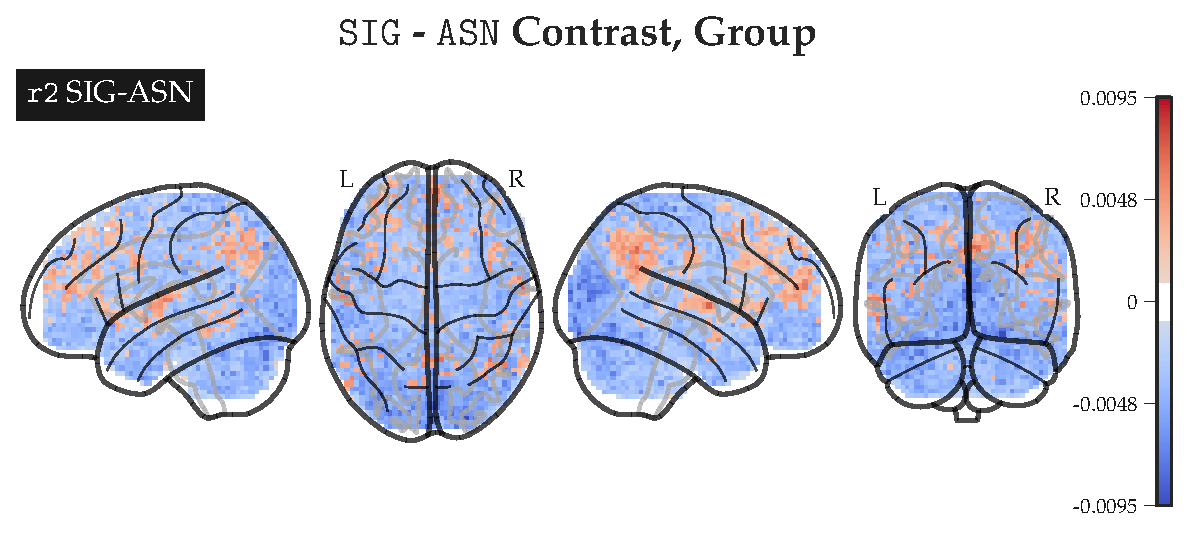
\includegraphics[width=.4\paperwidth]{Figures/EMB_SIG_ASN_r2_ContrastMapG.pdf}
    % % 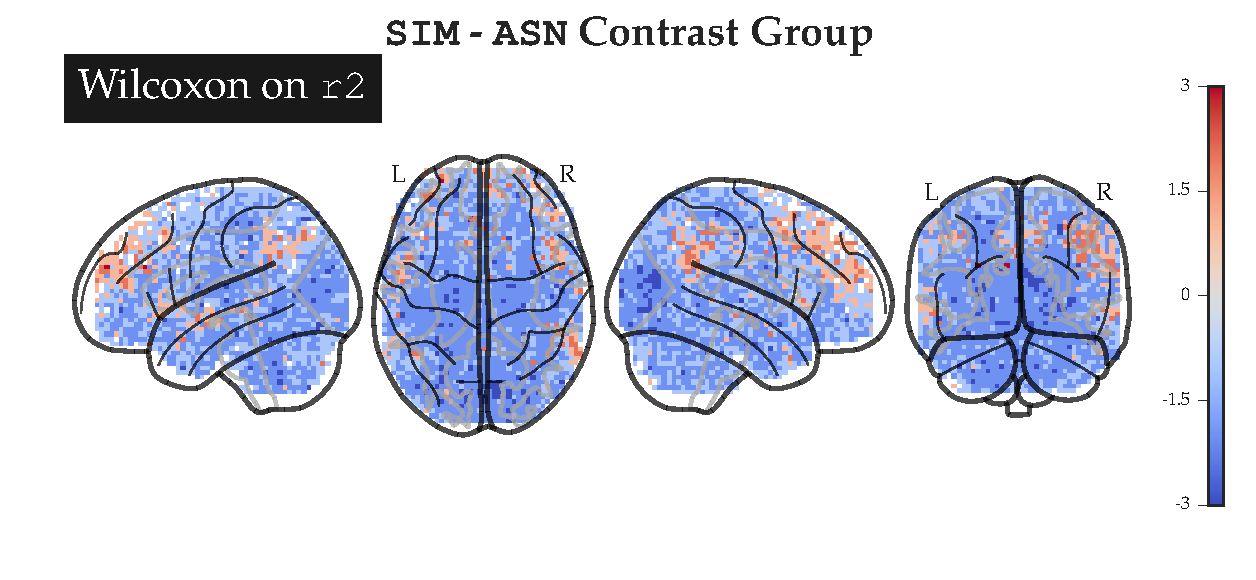
\includegraphics[width=.4\paperwidth, clip, trim=0cm,0cm,0cm, 1cm]{Figures/EMB_SIM_ASN_ContrastMapG.pdf}
    }
    % \end{minipage}
    % \begin{minipage}[t]{\textwidth}
    \makebox[\linewidth]{
        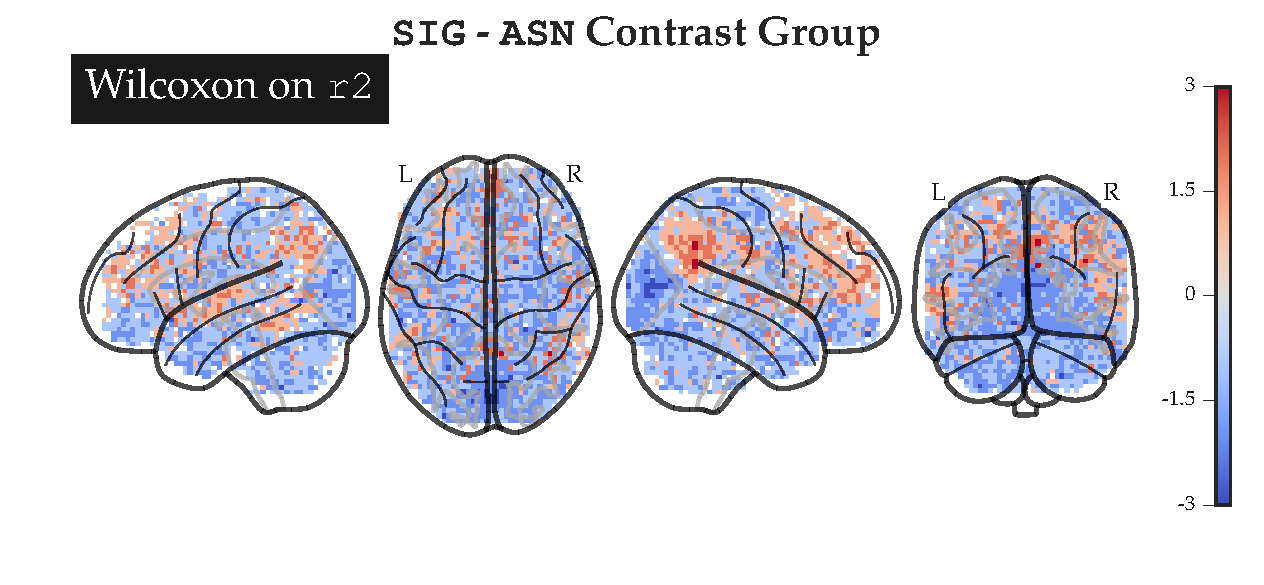
\includegraphics[clip, trim=0cm 0cm 0cm 1cm, width=.4\paperwidth]{Figures/EMB_SIG_ASN_ContrastMapG.pdf}
    }
    % \end{minipage}
    \caption[\code{SIG}-\code{ASN} Contrast, Group]{The differences of best voxel-model \code{r2}s are plotted in \textbf{upper panel}, significance levels in \textbf{lower panel}.} 
    \label{fig:EMB_SIG_ASN_ContrastMapG}
\end{figure}


\begin{figure}
    \centering
    \makebox[\linewidth]{
    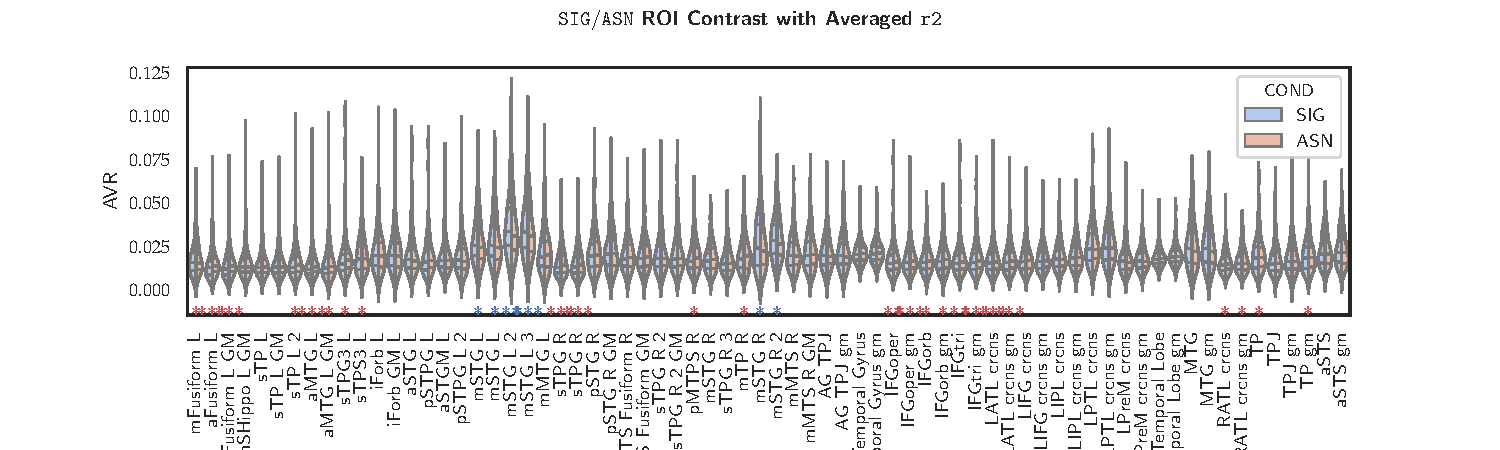
\includegraphics[width=\paperwidth]{Figures/SIG_ASN_ROI.pdf}
    }
    \caption[\code{SIG} \code{ASN} ROI Contrast, Group]{*: 0.05 uncorrected, ***: 0.05 ROI-wise multi-comparison corrected. Blue asterisks for \code{SIG}, red for \code{ASN}.\\ The average \code{r2} of voxels in a ROI is computed. We select only ROIs with scores>0.015 in either of \code{SIG} and \code{ASN} models. ROIs are of miminum size of 26 voxels (radius of 7 mm). Multiple ROIs in bilateral mSTG are found preferential for \code{SIG}, \code{ASN} are mostly inferiortemporal (including fusiform and hippocampal), anterotemporal (in TP and MTG) and inferofrontal in pars oper and triangularis.} 
    \label{fig:SIG_ASN_ROI}
\end{figure}
